%% %% %% %%
%%
%% Previo de la práctica
%%
%% %% %% %%

\documentclass[../main.tex]{subfiles}
\graphicspath{{\subfix{../images/}}}

\begin{document}
\section*{Previo}
\subsection*{Pregunta 1}
\begin{em}
  ¿Qué es un cronograma?
\end{em}

Se trata de la representación gráfica de un conjunto de señales de entrada y 
salida como funciones del tiempo. Debido a que dichas señales puede tomar 
únicamente valores de 0 y 1, su representación gráfica es una serie de pulsos 
cuadrados con diferentes longitudes. Las señales de entrada y salida se 
dibujan en el mismo diagrama para mostrar el comportamiento entrada-salida del 
sistema digital. Un cronograma muestra todos los posibles patrones de 
entrada-salida, no necesariamente en el mismo orden que la tabla de verdad.


\subsection*{Pregunta 2}
\begin{em}
  ¿Qué son las señales tipo Toggle, Random y Pulse?
\end{em}
\begin{itemize}
  \item \textbf{Toggle.} El término \textit{toggle} hace referencia a que 
    existe una conmutación. Es decir, se trata de una señal que sólo puede 
    tomar dos valores. Cada uno de estos valores representa un estado lógico.
  \item \textbf{Random.} Se trata de una señal que puede adquirir cualquier 
    valor en cualquier tiempo dado. Es decir, no existe algún patrón que se 
    repita en ella y no se pueden modelar con alguna función matemática.
  \item \textbf{Pulse.} Se trata de una señal que pasa de un estado inicial a 
    otro diferente en un intervalo determinado de tiempo finito; 
    posteriormente, retoma el valor inicial en otro intervalo de tiempo 
    finito.
\end{itemize}


\subsection*{Pregunta 3}
\begin{em}
  ¿Para qué se utiliza la resistencia Pull-Up o Pull-Down?
\end{em}

Se trata de resistencias dispuestas en un circuito de forma especial con la 
finalidad de establecer un estado lógico.
\begin{itemize}
  \item \textbf{Resistencia Pull Down.} En esta configuración la resistencia 
    tendrá una caída de potencial de $0 [V]$ de forma predeterminada 
    (\textit{LOW}); mientras que tendrá una caída de potencial de $V_{CC}$ en 
    caso contrario (\textit{HIGH}).

  \item \textbf{Resistencia Pull Up.} En esta configuración la resistencia 
    tendrá una caída de potencial de $V_{CC}$ de forma predeterminada 
    (\textit{HIGH}); mientras que tendrá una caída de potencial de $0$ en caso 
    contrario (\textit{LOW}).
\end{itemize}

\begin{figure}[H]
  \centering
  \begin{subfigure}[b]{0.45\textwidth}
    \centering
    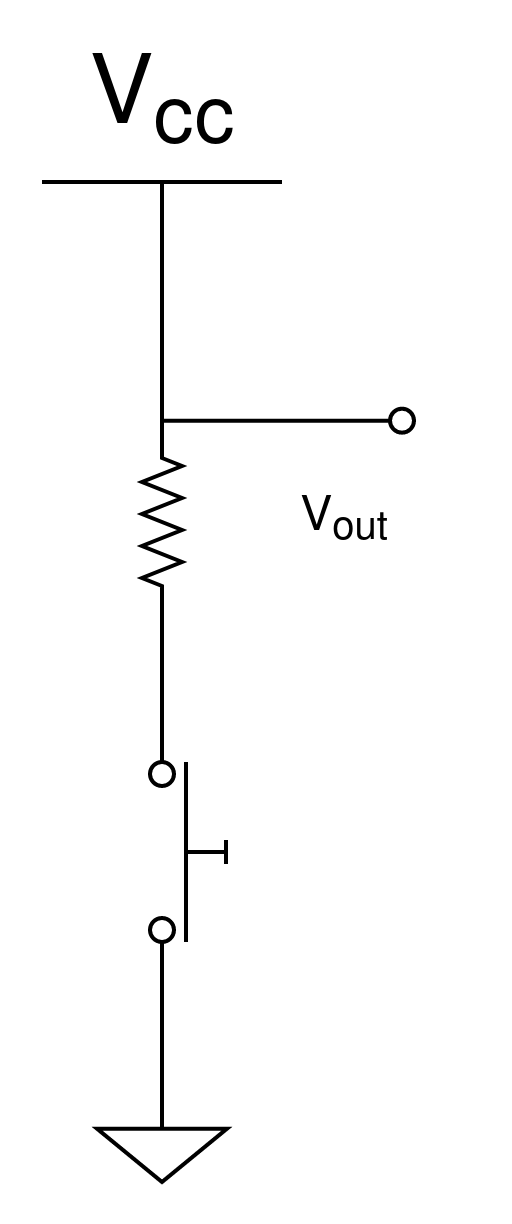
\includegraphics[height=7cm]{pull_down}
    \subcaption{\textit{Pull Down}}
  \end{subfigure}
  \hfill
  \begin{subfigure}[b]{0.45\textwidth}
    \centering
    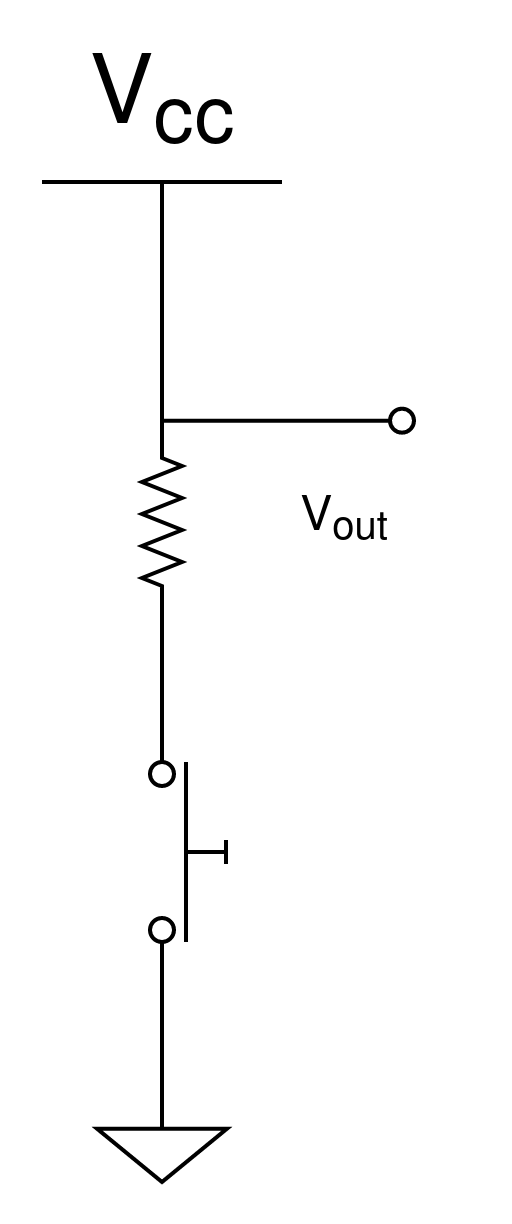
\includegraphics[height=7cm]{pull_up}
    \subcaption{\textit{Pull Up}}
  \end{subfigure}
  \caption{Resistencias \textit{Pull Up} y \textit{Pull Down}}
\end{figure}

\subsection*{Pregunta 4}
\begin{em}
  ¿Para un transistor a qué se le llama ``Corte'' y ``Saturación'' y cuál es su 
  efecto sobre las señales lógicas?
\end{em}

Se trata de dos regiones de operación de los transistores.
\begin{itemize}
  \item En la \textbf{región de corte}, ambas uniones del transistor están 
    polarizadas en sentido inverso, lo cual produce una corriente de colector 
    despreciable (para este caso, el transistor se comporta como un 
    interruptor abierto).
  \item En la \textbf{región de saturación}, ambas uniones del transistor 
    están polarizadas en directa, lo cual genera un crecimiento exponencial de 
    la corriente en el colector (para este caso, el transistor se comporta 
    como un interruptor cerrado).
\end{itemize}
Por lo tanto, se puede considerar un estado \textit{``on''} cuando el 
transistor está en la región de saturación y un \textit{``off''} cuando el 
transistor está en la región de corte.

\subsection*{Pregunta 5}
\begin{em}
  Analiza y caracteriza el siguiente circuito a través de cualquier simulador 
  e identifica el comportamiento que este tiene.
  \begin{itemize}
    \item Identifica el voltaje resultante en cada uno de los transistores 
      considerando que tanto la entrada A como B solamente pueden tener dos 
      voltajes (ground y $V_{CC}$), toda esta información colócala dentro de 
      una respectiva tabla y completa la misma.
  \end{itemize}
\end{em}

Para este caso, dentro del simulador se consideró un voltaje $V_{CC} = 5 [V]$, 
con lo cual se obtuvieron los siguientes valores:

\begin{table}[H]
  \centering
  \begin{tabular}{|p{1.5cm}|p{1.5cm}|p{1.5cm}|p{1.5cm}|p{1.5cm}|p{1.5cm}|}
    \hline
    \textbf{A}& \textbf{B}& \textbf{C}& \textbf{Q1}& \textbf{Q2}& \textbf{R2, Q3}  \\ \hline
    Ground  & Ground  & Ground  & 2.8     & 2.8     & 0       \\
    Ground  & Ground  & VCC     & 2.8     & 0       & 0       \\
    Ground  & VCC     & Ground  & 0       & 2.8     & 0       \\
    Ground  & VCC     & VCC     & 0       & 0       & 5       \\
    VCC     & Ground  & Ground  & 0       & 2.8     & 0       \\
    VCC     & Ground  & VCC     & 0       & 0       & 5       \\
    VCC     & VCC     & Ground  & 0       & 2.8     & 0       \\
    VCC     & VCC     & VCC     & 0       & 0       & 5       \\ \hline
  \end{tabular}
\end{table}


\end{document}

